\documentclass[12pt]{article}
\usepackage{graphicx}
\usepackage{caption}
\usepackage{subcaption}
\usepackage[T1]{fontenc}
\usepackage[scaled]{beramono}
%\renewcommand*\familydefault{\ttdefault}
\usepackage{listings}
 
\lstset{
  language=Python,
  showstringspaces=false,
  formfeed=\newpage,
  tabsize=4,
  commentstyle=\itshape,
  basicstyle=\ttfamily,
  morekeywords={models, lambda, forms}
}
 
\newcommand{\code}[2]{
  \hrulefill
  \subsection*{#1}
  \lstinputlisting{#2}
  \vspace{2em}
}

\begin{document}

\title{Error Analysis EAX}
\author{Kevin Chen}
\date{January 25, 2015}
\maketitle

\begin{obeylines}

\section{Problem 1}
{\footnotesize \textit{We want to measure the specific activity (number of decays per second) of a radioactive source so that we can use it to calibrate the equipment of the gamma-ray experiment. We use an electronic counter and a timer to measure the number of decays in a given time interval. In round numbers we measure 1000 decays in 5 minutes of observation. For how long should we measure in order to obtain a specific activity with a precision of 1\%? Explain.}}

Assuming that there are no instrumental time errors, the counts obey Poisson Statistics, and that we can expect another 1000 decays in the following 5 minutes, then to obtain a precision of 1\% we must have 10000 counts after 50 minutes. We obtain that result by the following Poisson characteristics: $$ \sigma = \sqrt{\mu} $$ $$ Precision = \frac{\sigma}{\mu} = \frac{\sqrt{\mu}}{\mu} = \frac{1}{\sqrt{\mu}} $$ $\mu$ then equals $$\frac{1}{Precision^2} = 100^2 = 10000 $$ To measure 10000 events, we need 50 minutes of time since we gather data at 200 events per minute.

\section{Problem 2}
{\footnotesize \textit{You are given two measurements of distance and their associated uncertainties: $A \pm \sigma_A$ and $B \pm \sigma_B$. Calculate the propagated uncertainty in the (a) total distance $A + B$, (b) difference $A - B$, (c) the perimeter $2A + 2B$ and (d) the area  $A \times B$ .}}

\begin{enumerate}
\item $ \sigma_{x, A+B} = \sqrt{\sigma_A^2 + \sigma_B^2} $
\item $ \sigma_{x, A-B} = \sqrt{\sigma_A^2 + \sigma_B^2} $ 
\item $ \sigma_{x, 2A+2B} = 2 \sqrt{\sigma_A^2 + \sigma_B^2} $
\item $ \sigma_{x, A \times B} = \sqrt{B\sigma_A^2 + A\sigma_B^2} $
\end{enumerate}
\end{obeylines}

\section{Problem 3}
{\footnotesize \textit{In this problem we will be generating and analyzing lists of normally distributed random numbers. The distribution we are sampling has true mean 0 and standard deviation 1. \begin{enumerate}
\item If we sample this distribution N=5 times, what do we expect the mean to be? How about the standard deviation? Whats the error on the mean?
\item Using Matlab, generate a list of N=5 normally distributed random numbers (the command randn(N,M) will generate M lists of length N). Calculate the mean, standard deviation and the error on the mean. Is this what you expected?
\item Now find the mean, standard deviation and error on the mean for M=1000 experiments of N=5 measurements each. Plot a histogram of the distribution. About how many experiments are within 1 sigma of the true mean of 0. About how many are within 2 sigma? Is this what you expected?
\item Now repeat questions 1-3 for N=10,50,100,1000. \end{enumerate}}}

For part 1 of this problem, I calculated the following means, standard deviations, and errors:
\begin{center}
  \begin{tabular}{|p{1cm}|p{2cm}|p{2cm}|p{2cm}|p{2cm}|p{2cm}|}
    \hline
    \textbf{Part} & \textbf{N = 5} & \textbf{N = 10} & \textbf{N = 50} & \textbf{N = 100} & \textbf{N = 1000}  \\ \hline
 1 & Mean=0 \newline SD=1 \newline {\footnotesize Err=$\frac{\sigma}{\sqrt{N}}$=$\frac{\sigma}{\sqrt{5}}$\newline=0.447} & 0 \newline 1 \newline 0.316 & 0 \newline 1 \newline 0.1414 & 0 \newline 1 \newline 0.1 & 0 \newline 1 \newline 0.0316  \\ \hline
\end{tabular}
\end{center}

For parts 2-4, I did not use MATLAB. Instead, I used Python and its numerical analysis package, NumPy. The following is the code I used to generate random numbers and the analysis for the mean, standard deviation, and error from the mean. 
\begin{lstlisting}
""" Python Code for Error Analysis Homework """

import numpy as np 
import math 
import matplotlib.pyplot as plt

def one_normal(n): # n = 5,10,50,100,1000
	measurements = np.random.standard_normal(n)
	mean = measurements.mean(axis = 0)
	std = measurements.std(axis = 0)
	mean_error = std / math.sqrt(n)
	print("Mean: " + str(mean))
	print("Standard Deviation: " + str(std))
	print("Error in the Mean: " + str(mean_error))

def normal(m,n): # m = 1000, n = 5,10,50,100,1000

	" Calculate the stats for the measurements per experiment. "
	experiments = np.random.randn(m,n)
	means = experiments.mean(axis = 1)
	standard_deviations = experiments.std(axis = 1)
	variances = [x*x for x in standard_deviations]
	errors = [x / math.sqrt(n) for x in standard_deviations]

	" Now calculate the stats of all the experiments. " 
	total_mean = sum(means)/m
	total_standard_deviation = math.sqrt(sum(variances))/m
	total_errors = total_standard_deviation/math.sqrt(m)
	print("Mean :" + str(total_mean))
	print("Standard Deviation: " + str(total_standard_deviation))
	print("Error :" + str(total_errors))
	plt.hist(means, 30)
	plt.show()
\end{lstlisting}

The follow figures display the analysis for Problem 3.2 and 3.3, along with the histograms for 3.3. 

\begin{figure}[ht]
	\centering
	\begin{minipage}[b]{0.47\linewidth}
		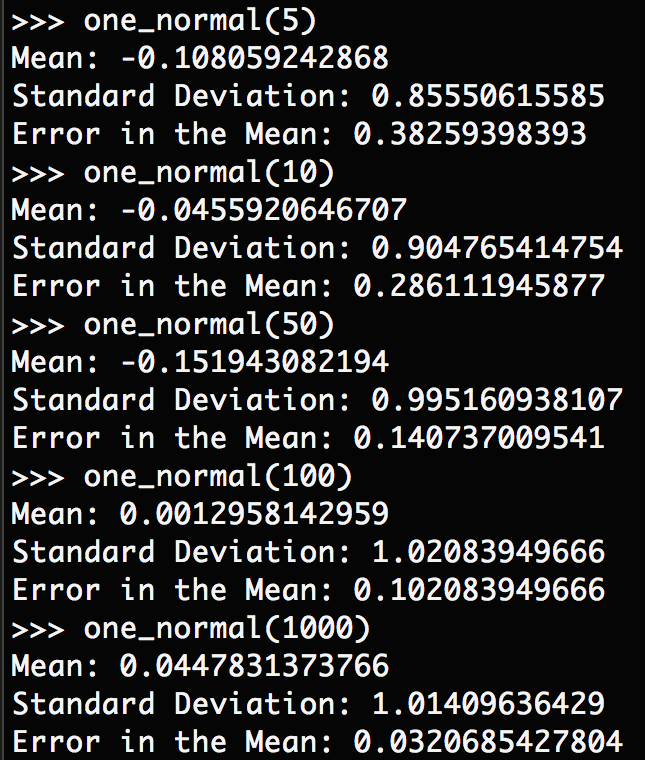
\includegraphics[width = 6cm]{P3_2.PNG}
		\caption{Analysis for Problem 3.2}
		\label{fig:minipage1}
	\end{minipage}
	\quad
	\begin{minipage}[b]{0.47\linewidth}
		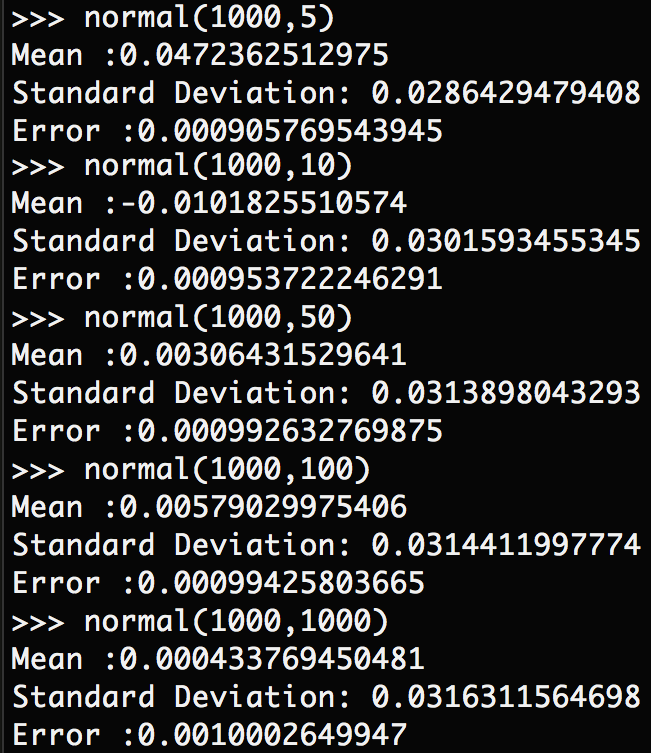
\includegraphics[width = 6cm]{P3_3.PNG}
		\caption{Analysis for Problem 3.3}
		\label{fig:minipage2}
	\end{minipage}
\end{figure}

\begin{figure}[ht]
	\centering
	\begin{minipage}[b]{0.47\linewidth}
		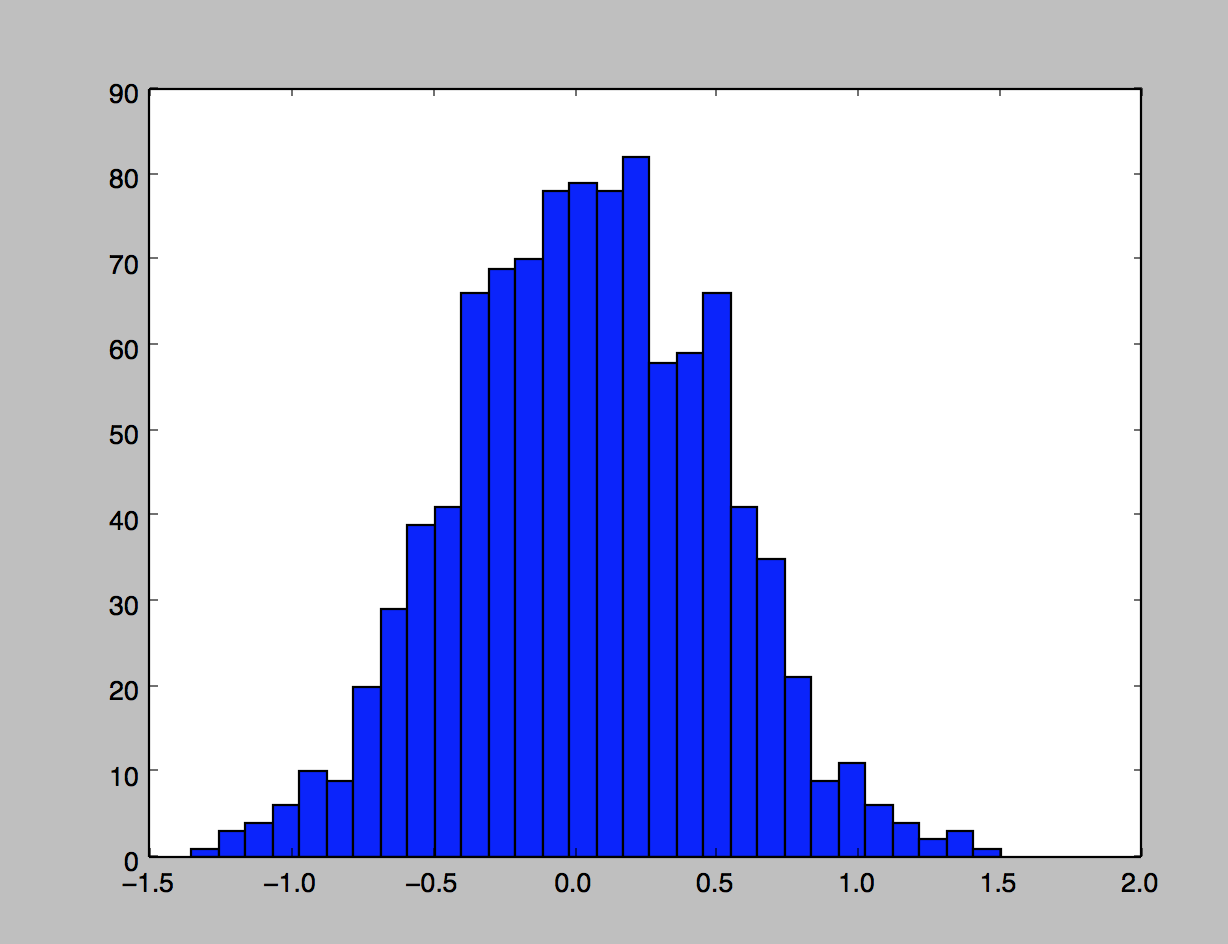
\includegraphics[width = 6cm]{P3N=5.png}
		\caption{Distribution of the means of 1000 experiments, each with 5 measurements}
		\label{fig:minipage1}
	\end{minipage}
	\quad
	\begin{minipage}[b]{0.47\linewidth}
		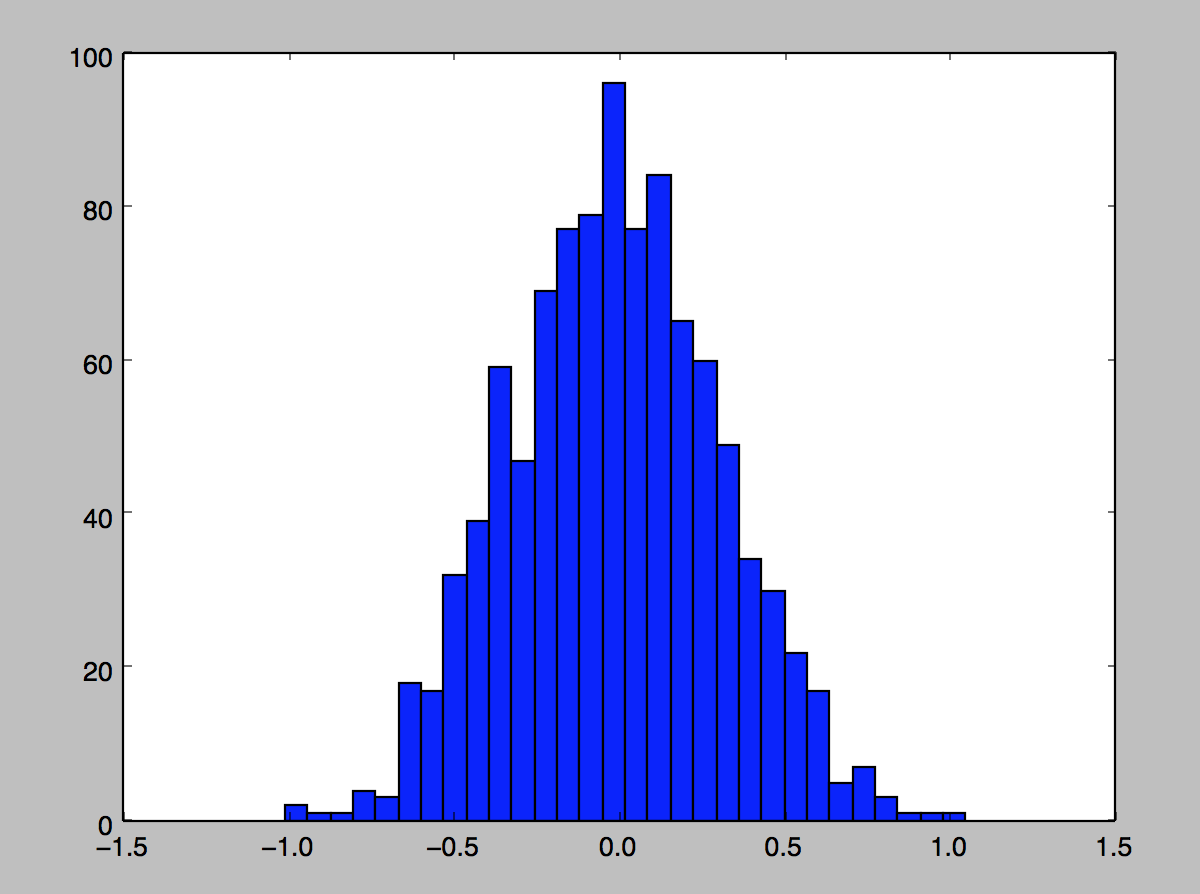
\includegraphics[width = 6cm]{P3N=10.png}
		\caption{Distribution of the means of 1000 experiments, each with 10 measurements}
		\label{fig:minipage2}
	\end{minipage}
\end{figure}

\begin{figure}[ht]
	\centering
	\begin{minipage}[b]{0.47\linewidth}
		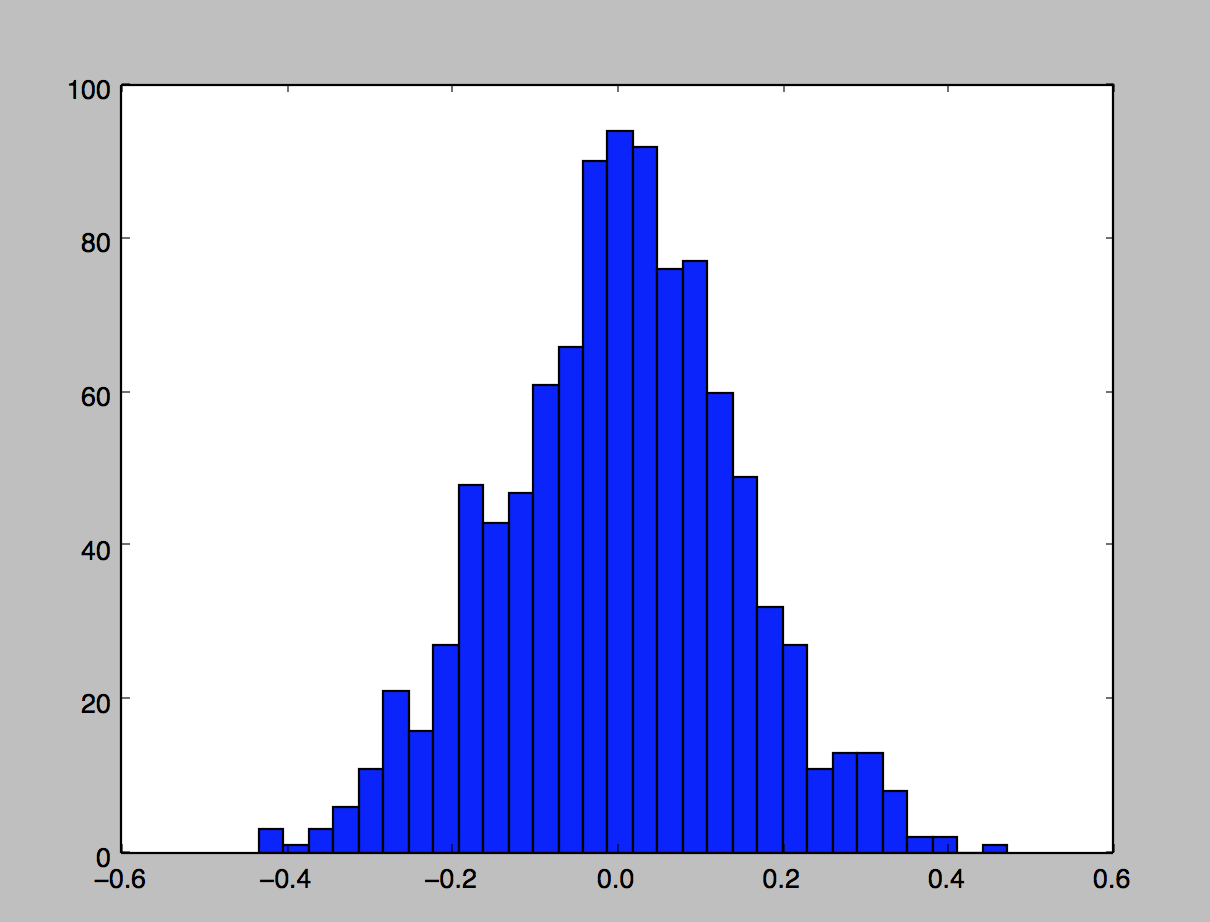
\includegraphics[width = 6cm]{P3N=50.png}
		\caption{Distribution of the means of 1000 experiments, each with 50 measurements}
		\label{fig:minipage1}
	\end{minipage}
	\quad
	\begin{minipage}[b]{0.47\linewidth}
		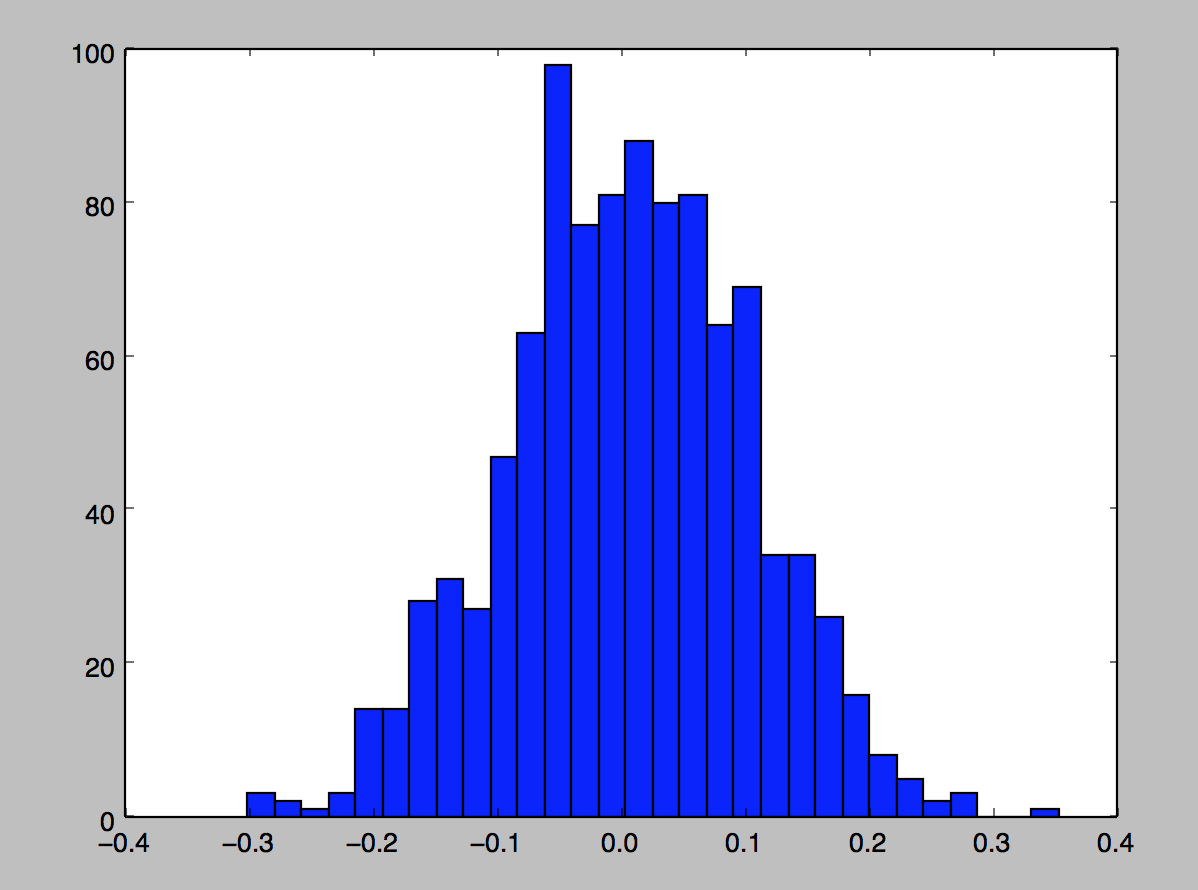
\includegraphics[width = 6cm]{P3N=100.png}
		\caption{Distribution of the means of 1000 experiments, each with 100 measurements}
		\label{fig:minipage2}
	\end{minipage}
\end{figure}

\begin{figure}[ht]
	\centering
	\begin{minipage}[b]{0.5\linewidth}
		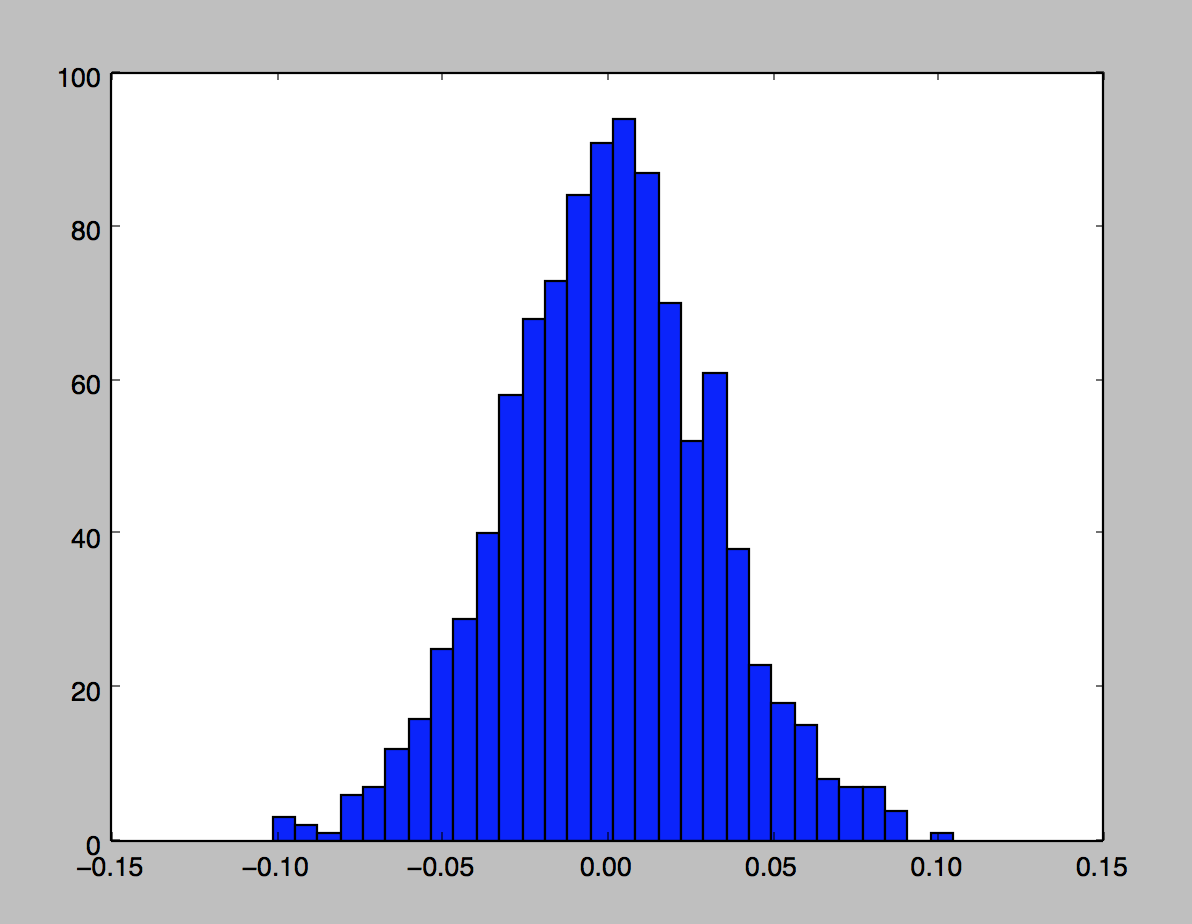
\includegraphics[width = 6cm]{P3N=1000.png}
		\caption{Distribution of the means of 1000 experiments, each with 1000 measurements}
		\label{fig:minipage1}
	\end{minipage}
	\quad
\end{figure}

\clearpage

\section{Problem 4}
{\footnotesize \textit{In this problem we will repeat the above process, but now using lists of exponentially distributed random numbers. The probability of selecting a random number between $x and x+dx is \propto e^{-x}dx.$ \begin{enumerate}
\item What do you expect to be the mean of the distribution? What do you expect to be the standard deviation? (Note: The standard deviation is defined exactly as it is for a normal distribution, but the 1 sigma = 68$\%$ rule no longer applies to a exponential distribution.) What do you expect to be the error on the mean for N=100? Given M=1000 lists of N=100 random numbers, what do you expect the distribution of means to look like? What is the error on the mean?
\item Make a list of N=100 exponentially distributed random numbers, (Hint: this can be easily done starting with a uniform distribution of random numbers.) Calculate the mean and standard deviation.
\item Make M=1000 lists of N=100 exponentially distributed random numbers. Make a histogram of the means. Does the distribution of means look as you thought? What is the standard deviation of the means. Does this agree with what you thought?
\item Repeat the previous steps for N=1000 and 10000. Does the error on the mean scale as you thought?\end{enumerate}
This is a demonstration of the Central Limit Theorem.}}

For part 1 of this problem, I calculated the following means, standard deviations, and errors:
\begin{center}
  \begin{tabular}{|p{1cm}|p{3cm}|p{2cm}|p{3cm}|}
    \hline
    \textbf{Part} & \textbf{N = 100} & \textbf{N = 1000} & \textbf{N = 10000}  \\ \hline
 1 & Mean=1 \newline SD=1 \newline {\footnotesize Err=$\frac{\sigma}{\sqrt{N}}$=$\frac{\sigma}{\sqrt{100}}$\newline=0.1} & 1 \newline 1 \newline 0.0316 & 1 \newline 1 \newline 0.01  \\ \hline
\end{tabular}
\end{center}
I expect the distribution for M=1000 and N={100,1000,10000} to approach a normal distribution. The error on that mean would be $\frac{standard deviation of exponentially distributed}{\sqrt(M)}$. 

For parts 2-4 of this problem, I used the following NumPy code to generate my random numbers. 
\begin{lstlisting}
""" Python Code for Error Analysis Homework """

import numpy as np 
import math 
import matplotlib.pyplot as plt

def one_exponential(n): # n = 100, 1000, 10000
	measurements = np.random.exponential(1,n)
	mean = measurements.mean(axis = 0)
	std = measurements.std(axis = 0)
	mean_error = std / math.sqrt(n)
	print("Mean: " + str(mean))
	print("Standard Deviation: " + str(std))
	print("Error in the Mean: " + str(mean_error))

def exponential(m,n): # m = 1000, n = 100, 1000, 10000

	" Calculate the stats for the measurements per experiment. "
	experiments = np.random.exponential(1,(m,n))
	means = experiments.mean(axis = 1)
	standard_deviations = experiments.std(axis = 1)
	variances = [x*x for x in standard_deviations]
	errors = [x / math.sqrt(n) for x in standard_deviations]

	" Now calculate the stats of all the experiments. " 
	total_mean = sum(means)/m
	total_standard_deviation = math.sqrt(sum(variances))/m
	total_errors = total_standard_deviation/math.sqrt(m)
	print("Mean: " + str(total_mean))
	print("Standard Deviation: " + str(total_standard_deviation))
	print("Error: " + str(total_errors))
	plt.hist(means, 30)
	plt.show()
\end{lstlisting}

For part 2, the calculated means and standard deviations are found in the terminal screenshots below, using the code from above. 

For part 3, the histograms, means, standard deviations, and errors on the mean are found in the terminal screenshots below. The distribution of means looks as I thought, just like a normal distribution. The standard deviation of the means does not follow the standard deviation of exponentially distributed numbers (which is just 1); instead, it follows that of a normal distribution. The standard deviation on the means is 0.0316, and seems to be approaching $1/\sqrt{M} = 1/\sqrt{1000}$.
 The follow figures display the analysis for Problem 4.2 and 4.3, along with the histograms for 4.3. As you can see, the Standard Deviations in 4.3 agrees with 4.1. 

For part 4, the N=1000 and N=10000 are accounted for in the pictures below. The error in the mean for 4.2 scales as I thought, which is by $1/\sqrt{N}$.

\begin{figure}[ht]
	\centering
	\begin{minipage}[b]{0.47\linewidth}
		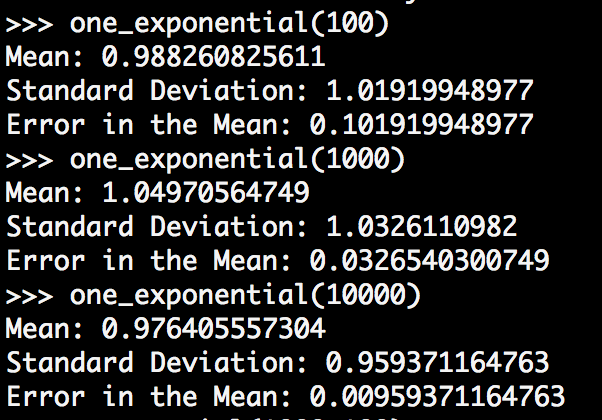
\includegraphics[width = 6cm]{P4_2.PNG}
		\caption{Analysis for Problem 4.2}
		\label{fig:minipage1}
	\end{minipage}
	\quad
	\begin{minipage}[b]{0.47\linewidth}
		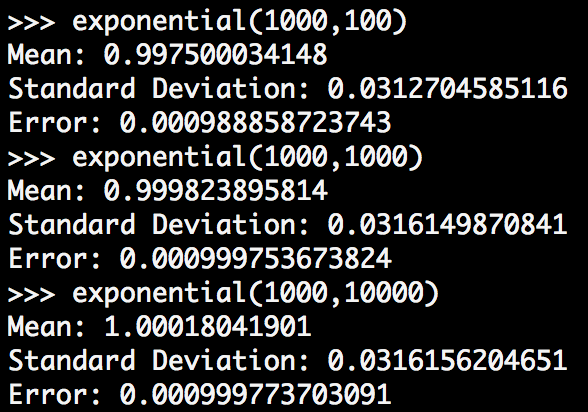
\includegraphics[width = 6cm]{P4_3.PNG}
		\caption{Analysis for Problem 4.3. Histograms are below.}
		\label{fig:minipage2}
	\end{minipage}
\end{figure}

\clearpage

\begin{figure}[ht]
	\centering
	\begin{minipage}[b]{0.47\linewidth}
		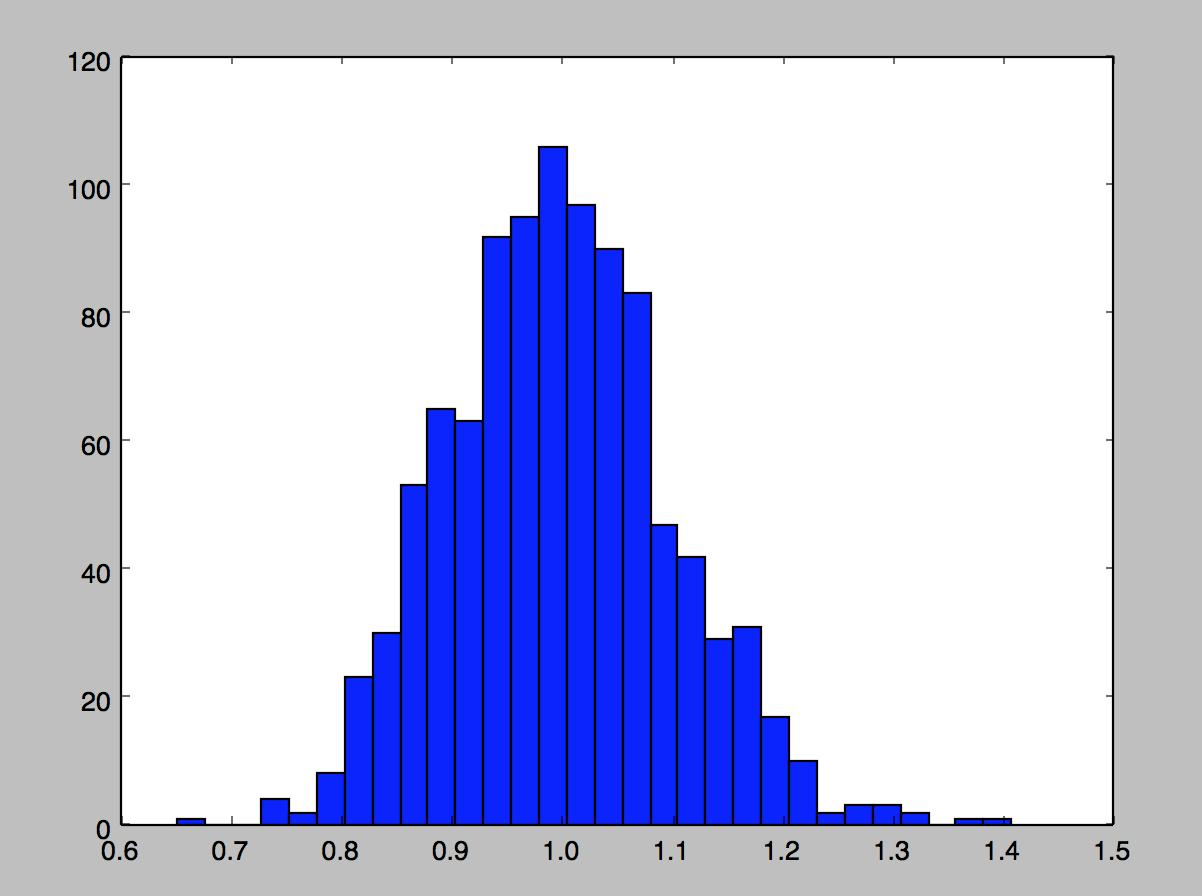
\includegraphics[width = 6cm]{ex N=100.png}
		\caption{Distribution of the means of 1000 experiments, each with 100 measurements}
		\label{fig:minipage1}
	\end{minipage}
	\quad
	\begin{minipage}[b]{0.47\linewidth}
		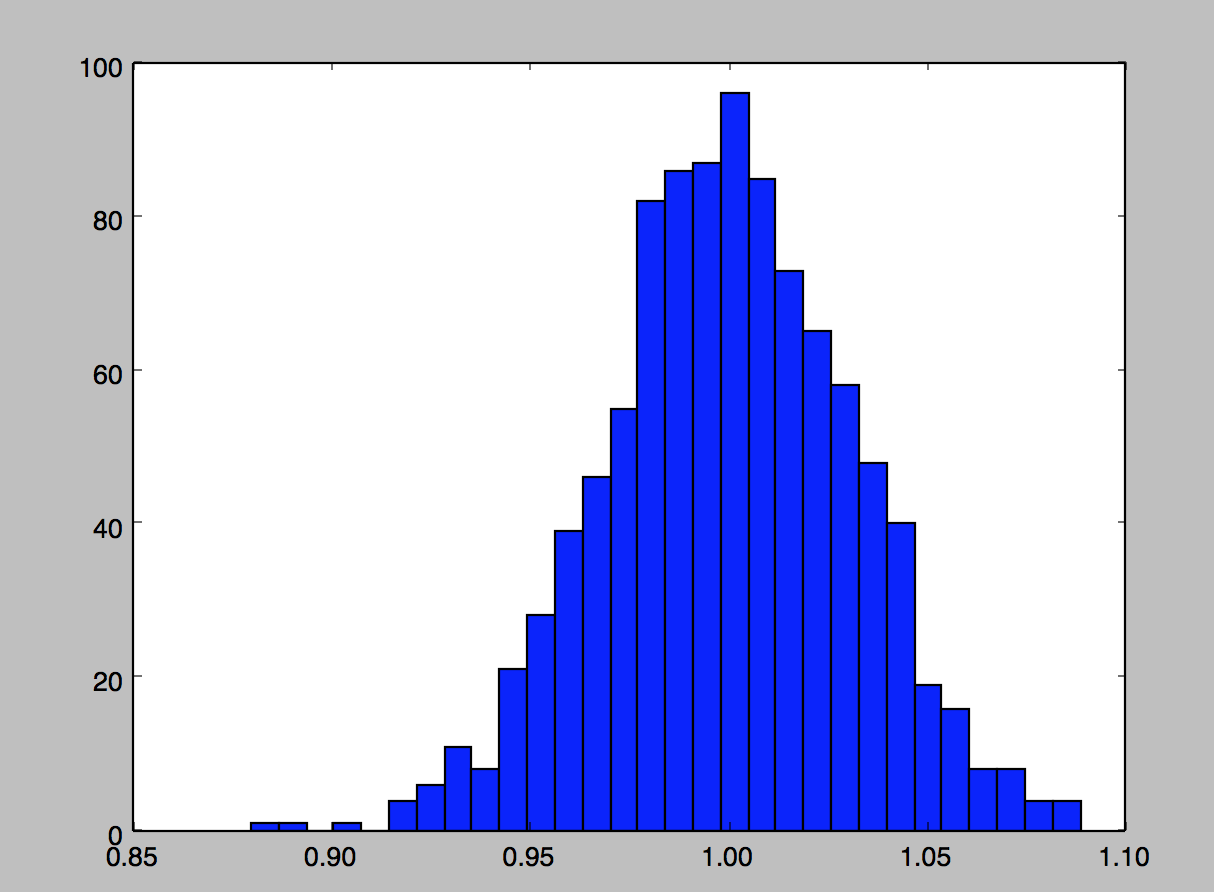
\includegraphics[width = 6cm]{ex N=1000.png}
		\caption{Distribution of the means of 1000 experiments, each with 1000 measurements}
		\label{fig:minipage2}
	\end{minipage}
\end{figure}

\begin{figure}[ht]
	\centering
	\begin{minipage}[b]{0.5\linewidth}
		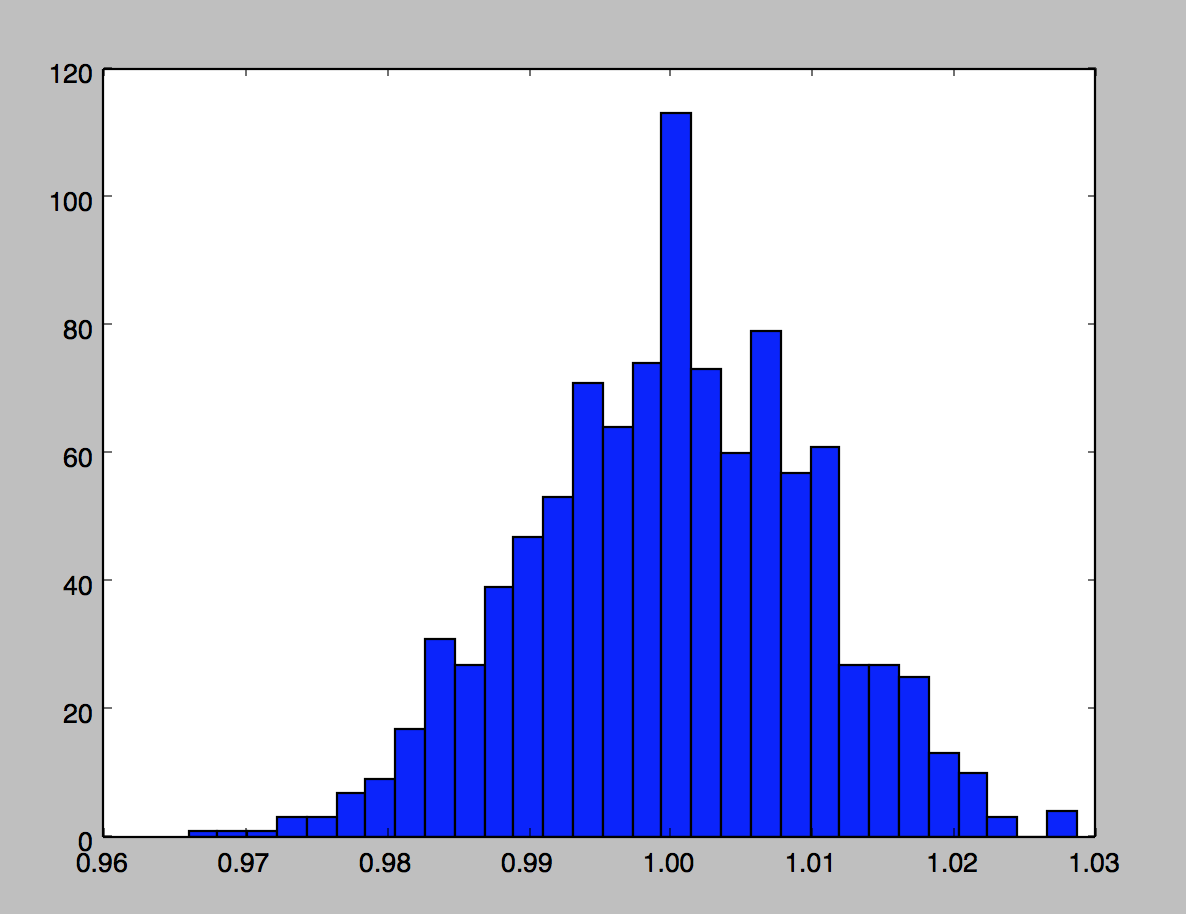
\includegraphics[width = 6cm]{ex N=10000.png}
		\caption{Distribution of the means of 1000 experiments, each with 1000 measurements}
		\label{fig:minipage1}
	\end{minipage}
	\quad
\end{figure}

\clearpage


\section{Problem 5}

\begin{figure}[h!]
  \caption{Peak.dat data.}
  \centering
    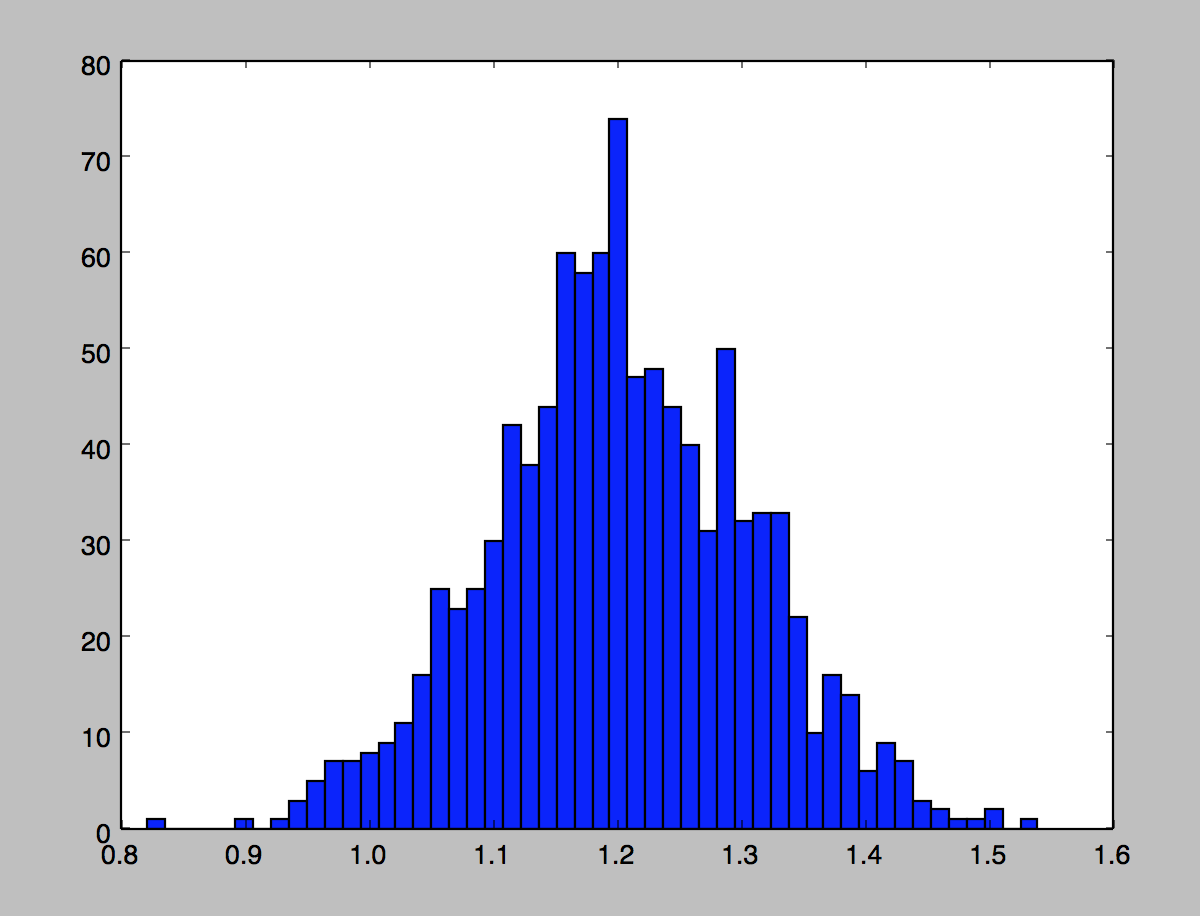
\includegraphics[width=12 cm]{peak.png}
\end{figure}


\begin{itemize}
	\item Above is the distribution of energies. I picked the 50 bins to get a nice compromise between granularity and high population in the most populated bin is relatively large. 
	\item The mean = 1.20, SD = 0.104, the error on the mean = 0.00328.
	\item I was not able to fit a Gaussian using NumPy. I will switch to MATLAB in the future since fitting curves in NumPy is excruciatingly difficult. 
	\item N/A
\end{itemize}

\clearpage

\section{Problem 6}
\begin{itemize}
	\item The slope is 3.05 and the intercept is 0.0397. See figure below.
	\item By using the formula for Chi-squared, we find the with an uncertainty of 0.01 MHz, we get a Chi-squared of 1520. The probability that this is an adequate fit is ~0. With an uncertainty of 1 MHz, we get a Chi-squared of 0.152. In the latter case the probably that the straight line is an adequate fit is 0.999. Therefore, we conclude that a good uncertainty is near 1MHz. 
	\item The uncertainty in the frequency is 0.12 MHz. The uncertainty in the intercept is about 0.067. The uncertainty in the slope is about 0.052. 
	\item With a weighted least-squares fit, the y-intercept is 0.0015 and the slope is 3.1. 
\end{itemize}

\begin{figure}[h!]
  \caption{Plot of the data with linear fit.}
  \centering
    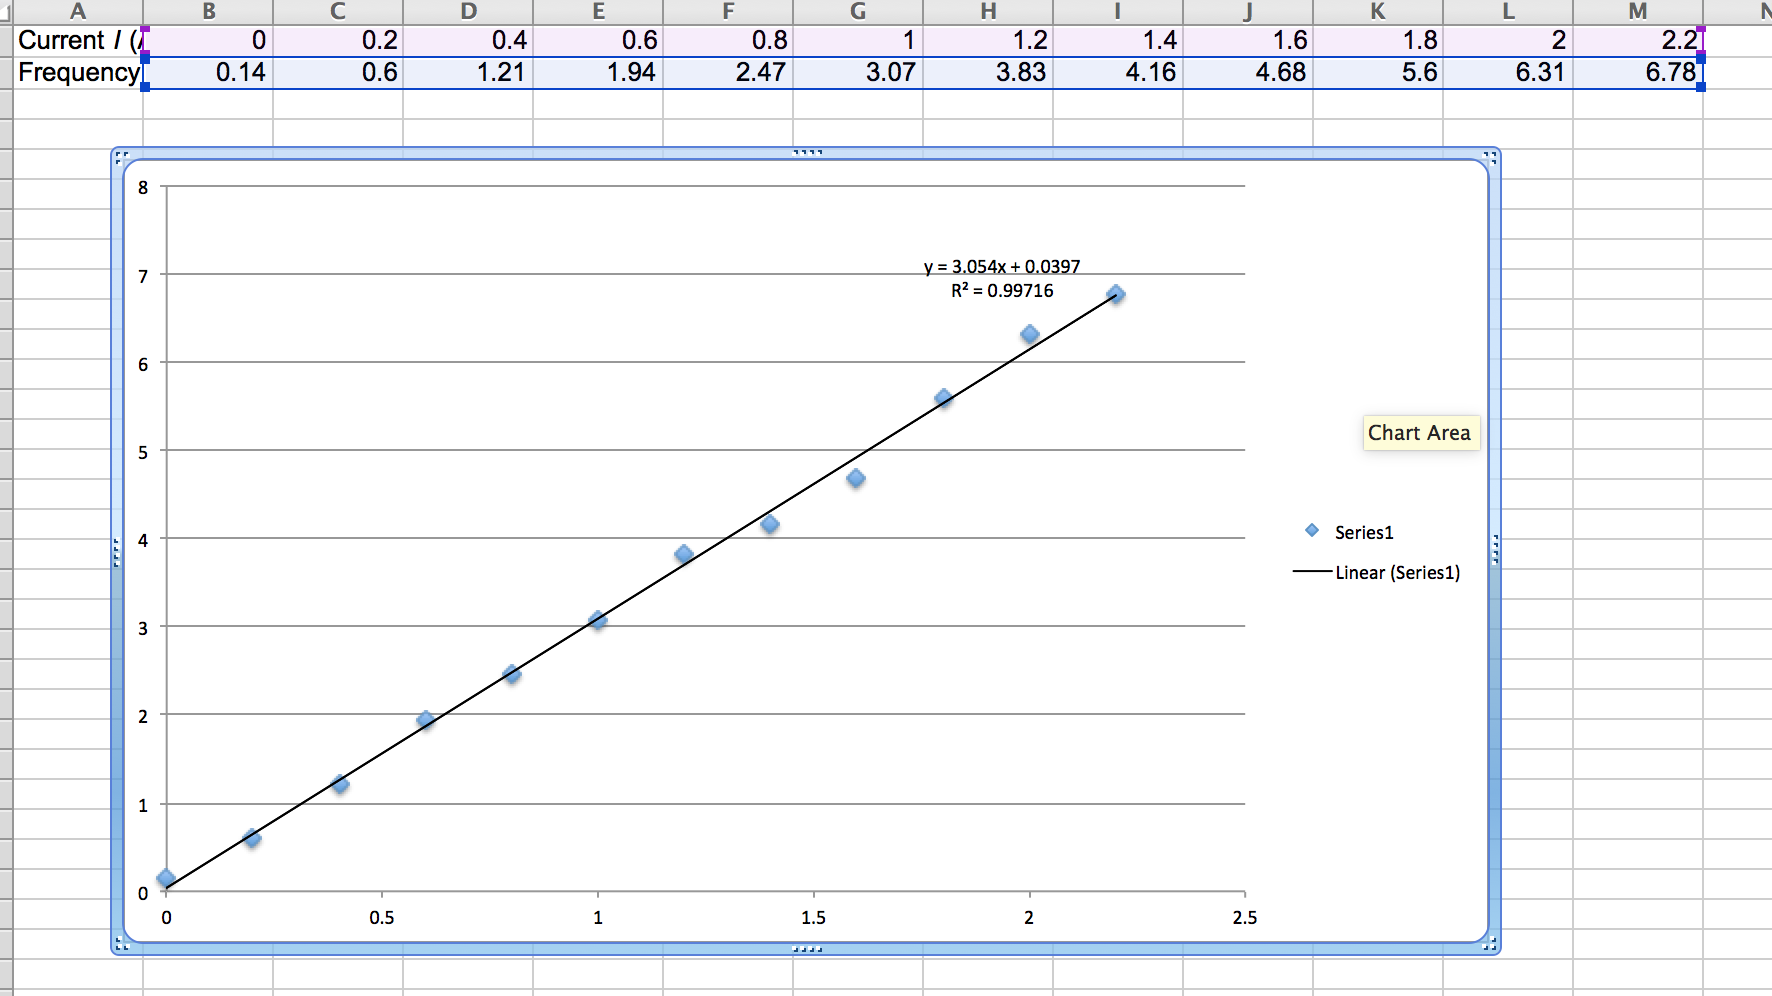
\includegraphics[width=15 cm]{linear_reg.png}
\end{figure}
\section{Problem 7}
\begin{itemize}
	\item The lower errors get larger and larger at the tail end of the exponential function due to the scaling of the y-axis. Quantitatively, the statistical error does not change. It is just the displaying of the error that changes. 
	\item $E_0 = \exp{2.1}=8.17$ and $\sigma_x = 0.5(E_0) = 4.08$ Note that these are extremely large experimental bounds. 
\end{itemize}


\end{document}






















